\section{Implementazione}

\subsection{Creazione del circuito}

\begin{frame}[fragile]{Normalizzazione dell'immagine}
	\begin{itemize}
		\item Normalizazione dell'immagine
		\begin{lstlisting}
def amplitude_encode(img_data):
	# Calculate the RMS value
	rms = np.sqrt(np.sum(np.sum(img_data**2, axis=1)))
	# Create normalized image
	image_norm = []
	for arr in img_data:
	for ele in arr:
	image_norm.append(ele / rms)
	# Return the normalized image as a numpy array
	return np.array(image_norm)

# Get the amplitude ancoded pixel values
image_norm_h = amplitude_encode(image)
		\end{lstlisting}
	\end{itemize}
\end{frame}

\begin{frame}[fragile]{Il circuito}
	\begin{itemize}
		\item Strutturazione
		\begin{lstlisting}[language=Python]
from qiskit import *
from qiskit import transpile
from qiskit_aer import Aer

# Create the circuit for horizontal scan
qc_h = QuantumCircuit(total_qb)
qc_h.initialize(image_norm_h, range(1, total_qb))
qc_h.h(0)
qc_h.unitary(D2n_1, range(total_qb))
qc_h.h(0)
		\end{lstlisting}
	\end{itemize}
\end{frame}

\begin{frame}[fragile]
	\begin{itemize}
		\item Immagine di esempio 16x16 in input
		\begin{figure}
			\centering
			\subfloat[Immagine originale]{%
			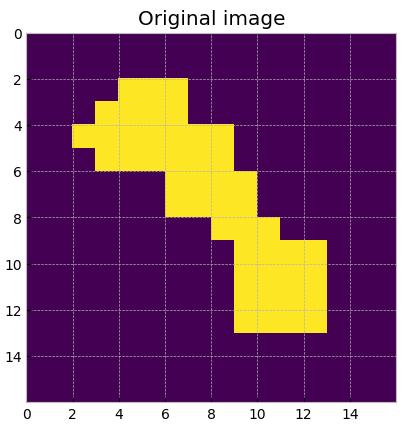
\includegraphics[width=0.4\textwidth]{16x16-original.png}%
			\label{fig:16x16-original}
			}
			\hfill
			\subfloat[Immagine normalizzata]{%
			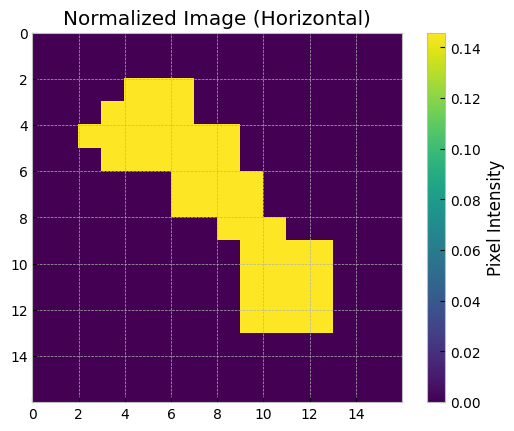
\includegraphics[width=0.5\textwidth]{16x16.png}%
			\label{fig:16x16-norm}
			}
			\caption{Confronto tra l'immagine originale (\ref{fig:16x16-original}) e l'immagine normalizzata (\ref{fig:16x16-norm}).}
		\end{figure}
	\end{itemize}
\end{frame}

\begin{frame}
	\begin{itemize}
		\item Circuito risultante
			\begin{figure}
				\centering
				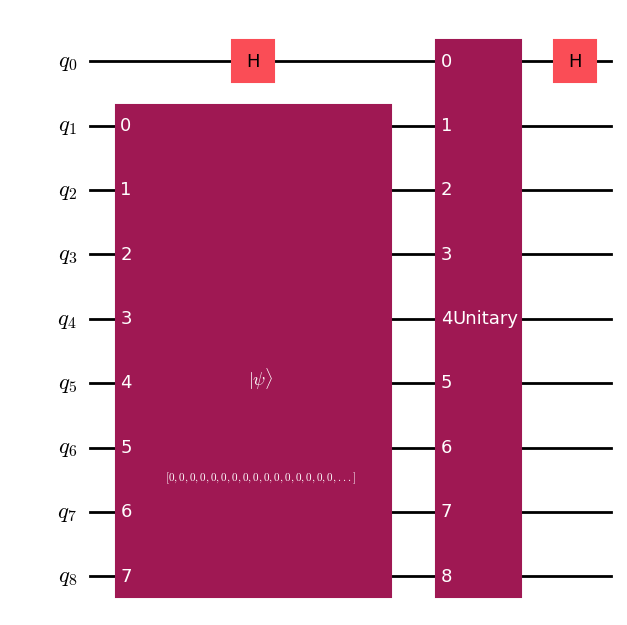
\includegraphics[width=0.65\textwidth]{16x16-circuit.png}
			\end{figure}
	\end{itemize}
\end{frame}

\begin{frame}{Codifica tramite gate}
	\begin{itemize}
		\item Per un'immagine 2x2
			\begin{figure}
				\centering
				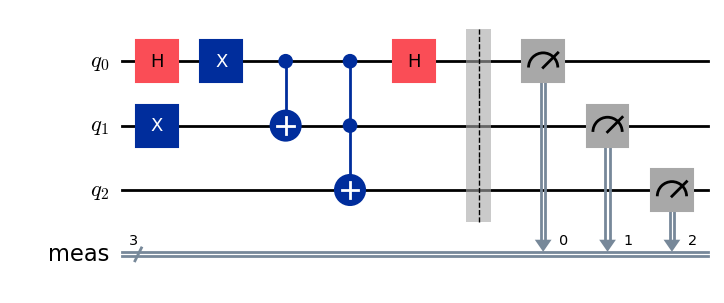
\includegraphics[width=0.8\textwidth]{2x2-transpiled.png}
			\end{figure}
	\end{itemize}
\end{frame}


\subsection{Error handling}

\begin{frame}[fragile]{La gestione degli errori}
	\begin{itemize}
		\item È stata utilizzata la classe \texttt{NoiseModel} di Qiskit
		\item Dati estrapolati dal backend reale \texttt{ibm\_kyiv}
		\begin{lstlisting}
from qiskit_aer import AerSimulator
from qiskit_aer.noise import NoiseModel

from qiskit_ibm_runtime import QiskitRuntimeService
service = QiskitRuntimeService(channel="ibm_quantum", token="XXX")

backend = service.backend("ibm_kyiv")
from qiskit_aer.noise import (NoiseModel, QuantumError, ReadoutError,
    pauli_error, depolarizing_error, thermal_relaxation_error)

noise_model = NoiseModel.from_backend(backend)
# Get coupling map from backend
coupling_map = backend.configuration().coupling_map
# Get basis gates from noise model
basis_gates = noise_model.basis_gates
		\end{lstlisting}
	\end{itemize}
\end{frame}

